\providecommand*{\lstnumberautorefname}{line}

High-level Synthesis tools, like LegUp or VivadoHLS, can automatically generate a circuit
for the matrix multiplication example in Listing \ref{lst:MMM}.
What if the designer was required to run this circuit reliably in the
presence of soft errors? 
The naive approach would be to instantiate multiple copies and each copy would run in lock-step
on the same input data and any deviation between them would indicate an error.

\lstset{language=C}
\begin{lstlisting}[basicstyle=\ttfamily\footnotesize, frame=single, label={lst:MMM}, captionpos=b, caption={Matrix Multiplication Example},numbers=left,escapeinside={@}{@}]
void MMM(float A[5][5],float B[5][5],float C[5][5])
{ int i=0, j=0, k=0;
  for(i=0, i<5, i++){
    for(j=0, j<5; j++){
      C[i][j] = 0;
      for(k=0, k<5; k++){
        @\label{lst:MMM_2}@C[i][j] += A[i][k]*B[k][j]; }
    }
  }
}
\end{lstlisting}

However replication in this fashion is expensive in both area and more importantly
power. 
Figure \ref{fig:singleHLSArch} provides a diagram of the resulting
circuit with two clear partitions, a data path where functional units reside, and a
control FSM responsible for scheduling instructions onto the functional units. 
Duplicating or even triplicating this design naively would dramatically increase the
area, especially as expensive floating point arithmetic units are required for the
calculation of the inner dot product. 

\begin{figure}[h]
\centering
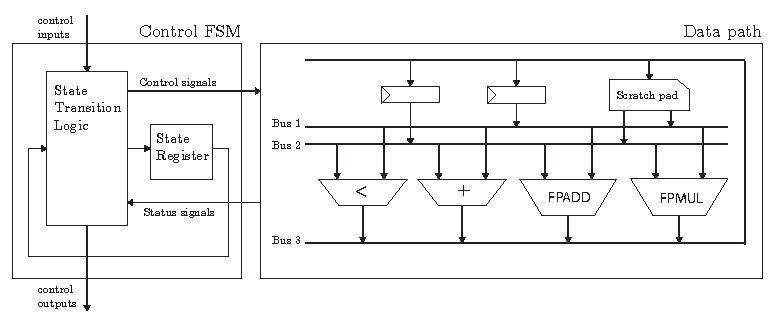
\includegraphics[width=3.5in]{./imgs/singleHLSArch.pdf}
\caption{Diagram representing a HLS circuit for the Matrix Multiplication example}
\label{fig:singleHLSArch}
\end{figure}

%Reliability and productivity are challenging issues
%currently effecting the design of VLSI/FPGA systems as
%device density increases.
%Addressing the latter issue High Level Synthesis (HLS) tools \cite{canis2011legup} have
%been both commercially and academically successful at trading
%performance for productivity, however their generated circuits are not reliable.
%To generate reliable circuits engineers are often faced with either:
%full circuit replication, which can be easily automated with tools but
%is expensive in resource or power costs; or expend considerable
%effort manually designing a reliable circuit.
%
%For reliable execution do we need full replication?
%From reviewing the literature you would quickly discover the answer
%is often application dependant but that for a significant number
%there are distinct regions of critical and non-critical code,
%especially in cases involving media processing or machine
%learning\cite{wong2006soft} \cite{liu2012flikker}.
%In this paper we argue that it is often the case that instructions important to the control flow of an application are more critical
%than instructions that only effect data; for example, an image renderer which can tolerant errors within
%it's pixel values but errors in it's control flow could cause it to hang indefinitely \cite{sampson2011enerj}.
%
%%\subsection{Matrix Multiplication Example}
%To demonstrate and highlight the potential saving that duplicating just
%the control flow can achieve we will use an example of HLS circuit generated from a
%matrix multiplication C function in \hyperref[lst:MMM]{Listing \ref{lst:MMM}}.
%A representation of the generated circuit can be seen in Figure \ref{fig:singleHLSArch}
%depicting the dataflow section containing functional units, and the
%control FSM responsible for scheduling instruction execution on functional units.
%
%
%\begin{figure}[h]
%\centering
%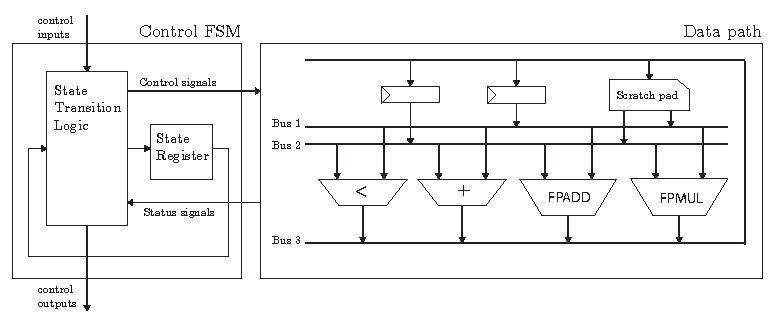
\includegraphics[width=3.5in]{./imgs/singleHLSArch.pdf}
%\caption{Diagram representing a HLS circuit for the Matrix Multiplication example}
%\label{fig:singleHLSArch}
%\end{figure}
%%The HLS generated circuit for this function can be divided into two main subsystems, a datapath, and a control FSM.
%%Within the datapath are all the functional units required to perform the computation, which in our example will contain:
%%integer comparators and incrementers for calculating the loop conditionals; and floating point adders and multipliers
%%for computing line \autoref{lst:MMM_2} of Listing \ref{lst:MMM}.
%%As the control FSM contains logic used for scheduling which operation is performed on a functional unit in the datapath,
%%when that operation is performed, and how data is moved between functional units.
%
%If this circuit was operating in the presence of soft errors then upsets within
%the floating point addition and multiplication circuitry used to calculate line \ref{lst:MMM_2} could potentially cause the data in the output
%matrix to be incorrect.
%As errors in the integer functional units effecting lines 3,4 and 6
%could cause the calculation of rows and columns of the output matrix \lstinline$C$ to be skipped, or even
%worse, cause the circuit to enter an infinite loop and never terminate.
%
%Let's say in this case errors in
%the output are tolerable or can be detected through statistical means at a later point, but
%there is a strict requirement that the circuit finishes in correct number of cycles and must
%always terminates.
%Initially we might try the industry standard of full circuit replication
%but due to the expensive replication of the floating point units it is infeasible in both area and power.
%Since we only need to ensure that the circuit takes the appropriate cycles,
%we might try and duplicate just the control FSM however this wont work since state transitions
%within the control FSM are dependant on the outputs of results in the datapath.
%Eventually we realise that by removing the floating point units from the datapath
%it is  possible to protect all the control decisions of the program while reducing the amount of resources required
%to do so.
%
%Manual inspecting code and removing elements that don't influence control flow
%may be feasible in the simple case of Matrix Multiplication, however as the complexity of the input increases
%the engineering effort required in both analysing the input source and generating circuits with an identical control FSM is
%significant.
%StitchUp fully automates this process through using a static analysis technique, known as program slicing, to extract
%and duplicate any instructions that may influence control.
%
%The contribution of this paper are:
%\begin{itemize}
%\item StitchUp, a tool which can automatically extract and protect the control flow structure of a circuit generated with a HLS tool.
%\item Detailed results of the CHStone benchmark, where exhaustive fault injection is performed on the majority of circuits.
%\item Results exploring the reliability of StitchUp protected circuits as the control to data ratio is varied through
%loop unrolling in the matrix multiplication example.
%
%\end{itemize}


